%%%%%%%%%%%%%%%%%%%%%%%%%%%%%%%%%%%%%%%%%%%%%%%%%%%%%%%%%%%
% --------------------------------------------------------
% Rho
% LaTeX Template
% Version 2.1.1 (01/09/2024)
%
% Authors: 
% Guillermo Jimenez (memo.notess1@gmail.com)
% Eduardo Gracidas (eduardo.gracidas29@gmail.com)
% 
% License:
% Creative Commons CC BY 4.0
% --------------------------------------------------------
%%%%%%%%%%%%%%%%%%%%%%%%%%%%%%%%%%%%%%%%%%%%%%%%%%%%%%%%%%%

\documentclass[9pt,a4paper,twoside]{rho-class/rho}
\usepackage[english]{babel}
\usepackage{amsmath}
% \usepackage{algorithmic} % Añade esto en el preámbulo
\usepackage{algorithm}
\usepackage{algpseudocode}
\usepackage{hyperref} % Para manejar URLs
\usepackage{biblatex} % Para el manejo de bibliografía
\usepackage{booktabs}
\usepackage{siunitx}
\usepackage{multirow}

\addbibresource{rho.bib} 

%% Spanish babel recomendation
% \usepackage[spanish,es-nodecimaldot,es-noindentfirst]{babel}

\setbool{rho-abstract}{true} % Set false to hide the abstract
\setbool{corres-info}{false} % Set false to hide the corresponding author section

%----------------------------------------------------------
% TITLE
%----------------------------------------------------------

\journalname{Practica 02}
\title{ Análisis Comparativo: Simulated Annealing vs Hill Climbing en la Optimización de Portafolios Financieros }

%----------------------------------------------------------
% AUTHORS AND AFFILIATIONS
%----------------------------------------------------------

% \author[1]{Alberto Valentín Velásquez Santos}
% \author[2]{Rodolfo Morocho Caballero}
% \author[3]{Max Houston Ramirez Martel}
% \author[4]{Harold Mondragon Tavara}
\author[,$\dagger$]{Alberto Valentín Velásquez Santos}
\author[,$\dagger$]{Harold Mondragon Tavara}
\author[,$\dagger$]{Max Houston Ramirez Martel}
\author[,$\dagger$]{Rodolfo Morocho Caballero}


%----------------------------------------------------------

% \affil[1]{Alberto Valentín Velásquez Santos}
% \affil[2]{Rodolfo Morocho Caballero}
% \affil[3]{Max Houston Ramirez Martel}
% \affil[4]{Harold Mondragon Tavara}
\affil[$\dagger$]{Estos autores contribuyeron igualmente a este trabajo.}
%----------------------------------------------------------
% DATES
%----------------------------------------------------------
\dates{Este archivo fue compilado el 13 de noviembre del 2024}

%----------------------------------------------------------
% FOOTER INFORMATION
%----------------------------------------------------------

\leadauthor{Group The Bankers}
\footinfo{Creative Commons CC BY 4.0}
\smalltitle{\LaTeX\ Template}
\institution{Universidad de Tecnologia E Ingeniería}
\theday{\DTMnow} %\today

%----------------------------------------------------------
% ARTICLE INFORMATION
%----------------------------------------------------------

% \corres{Provide the corresponding author information and publisher here.}
% \email{example@organization.com.}
% \doi{\url{https://www.doi.org/exampledoi/XXXXXXXXXX}}

\received{noviembre 13, 2024}
\revised{noviembre 13, 2024}
\accepted{noviembre 13, 2024}
\published{noviembre 13, 2024}
\license{Rho LaTeX Class \ccLogo\ This document is licensed under Creative Commons CC BY 4.0.}

%----------------------------------------------------------
% ABSTRACT
%----------------------------------------------------------

\begin{abstract}
    Este trabajo busca analizar y comparar la efectividad de dos algoritmos de optimización – Simulated Annealing y Hill Climbing – en el contexto de la optimización de portafolios financieros. Se utilizará el Sharpe Ratio como función fitness para medir el rendimiento ajustado al riesgo de los portafolios generados por cada algoritmo. El objetivo es identificar las ventajas y limitaciones de ambos métodos en términos de su capacidad para maximizar el rendimiento ajustado al riesgo en un conjunto de datos de activos financieros. Comparar Simulated Annealing y Hill Climbing en el contexto de la optimización de portafolios resulta relevante, ya que ambos algoritmos ofrecen enfoques distintos  para la búsqueda de soluciones óptimas. Simulated Annealing explora el espacio de soluciones con una mayor capacidad para evitar los óptimos locales debido a su proceso de "enfriamiento", lo que podría ofrecer soluciones potencialmente superiores para problemas complejos como la optimización de portafolios. Por otro lado, Hill Climbing es conocido por su mayor velocidad, aunque puede quedar atrapado en óptimos locales, lo cual es una desventaja en contextos de alta variabilidad y múltiples picos en la función objetivo. La comparación de estos dos enfoques proporcionará una perspectiva sobre la eficiencia y aplicabilidad de cada algoritmo en la gestión de portafolios ajustada al riesgo.
\end{abstract}

%----------------------------------------------------------

\keywords{optimización, heurísticas, Simulated Annealing, Hill Climbing , Machine Learning, Markowitz}
%----------------------------------------------------------

\begin{document}
	
%----------------------------------------------------------
% OPTIMIZATION PROBLEMS
%---------------------------------------------------------- 
    \maketitle
    \section{Marco Teórico}

        \rhostart{L}a optimización de portafolios es una práctica central en las finanzas, enfocada en maximizar el rendimiento ajustado al riesgo de una cartera para un nivel de riesgo dado, o en minimizar el riesgo para un rendimiento específico. Este proceso se fundamenta en los principios de diversificación y equilibrio entre riesgo y retorno, tal como se describe en la teoría de portafolios de Markowitz (1952) \cite{Markowitz1952}, que sentó las bases para el análisis moderno de inversiones. En este modelo, la minimización de la varianza de los retornos se combina con la maximización de su media para construir una cartera eficiente, definiendo el riesgo como la volatilidad de los retornos de una cartera y permitiendo que los inversores tomen decisiones informadas en función de su tolerancia al riesgo.

        Complementando la teoría de Markowitz, el Sharpe Ratio, introducido por William F. Sharpe en 1966, evalúa la eficiencia de una cartera ajustando su rendimiento al riesgo (Sharpe, 1966)\cite{Sharpe1966}. Este ratio es calculado dividiendo el exceso de retorno de la cartera sobre la tasa libre de riesgo por la desviación estándar de sus retornos. De esta manera, el Sharpe Ratio permite una comparación directa entre carteras al normalizar los retornos en términos del riesgo asumido, consolidándose como una herramienta fundamental para la optimización de portafolios en el ámbito financiero, especialmente cuando se busca maximizar la recompensa obtenida por cada unidad de riesgo.
        
        La optimización de portafolios implica complejidades adicionales cuando se introducen restricciones no lineales, como los costos de transacción fijos o los límites en la inversión en unidades discretas. Estas restricciones convierten el problema en uno no convexo, limitando la efectividad de los métodos clásicos como la programación cuadrática y lineal. En este contexto, los algoritmos heurísticos como Hill Climbing (HC) y Simulated Annealing (SA) han surgido como alternativas viables para enfrentar la naturaleza de estas funciones objetivo. HC es un algoritmo de búsqueda local que optimiza la función objetivo mediante ajustes incrementales a una solución inicial. Aunque es rápido en converger hacia un óptimo local, su enfoque determinista lo hace vulnerable a quedar atrapado en estos óptimos, lo que puede ser un obstáculo significativo en problemas complejos de optimización de portafolios, donde las múltiples restricciones generan una superficie de solución con múltiples picos y valles. Simulated Annealing (SA), que permite una exploración más amplia del espacio de soluciones al aceptar soluciones subóptimas en las primeras etapas del proceso. Este enfoque de exploración adaptativa evita que el algoritmo se quede atrapado en óptimos locales, permitiendo una búsqueda más robusta de soluciones óptimas globales, especialmente en problemas de optimización no convexos, como aquellos que incluyen costos fijos de transacción. En el estudio de Rubio-García, García-Ripoll y Porras (2022)\cite{Rubio-Garcia2022}, se evidencia que SA es particularmente adecuado para la optimización de portafolios en presencia de restricciones complejas. Su estructura estocástica y adaptativa permite reducir el tiempo de búsqueda al explorar eficientemente soluciones subóptimas al inicio, lo que contribuye a la eficacia de este algoritmo en problemas de portafolios discretos. Además, el estudio introduce una métrica de rendimiento denominada "time to target" (tiempo para alcanzar el objetivo), que cuantifica el tiempo requerido para obtener una solución de calidad en términos de una solución que maximiza el Sharpe Ratio, proporcionando una referencia para comparar la eficiencia de SA frente a otros métodos.
        
        En la comparación entre Hill Climbing y Simulated Annealing, este último muestra una capacidad superior para maximizar el Sharpe Ratio al ser más resistente a los óptimos locales. Esto es esencial en escenarios financieros donde la complejidad de las restricciones y los costos fijos de transacción agregan un nivel adicional de dificultad. Hill Climbing, si bien eficiente en tiempo, resulta limitado en su exploración y podría no encontrar la solución óptima global en problemas de portafolios que incluyen estos componentes no convexos. En este sentido, el uso de SA ofrece una exploración del espacio de soluciones más completa, mientras que Hill Climbing es preferible en situaciones donde se prioriza la rapidez de convergencia sobre una búsqueda exhaustiva.
        
    
    \section{Metodología fitness restricciones}
            
            Para evaluar el desempeño de Simulated Annealing y Hill Climbing en la optimización de portafolios, este estudio emplea el Sharpe Ratio como función fitness. El Sharpe Ratio, definido anteriormente como la diferencia entre el rendimiento esperado del portafolio y la tasa libre de riesgo, dividido por la desviación estándar de los rendimientos, es un indicador clave en la gestión de inversiones, pues permite medir la eficiencia de una cartera en términos de retorno ajustado al riesgo. Utilizar el Sharpe Ratio como objetivo de optimización permite que ambos algoritmos ajusten la composición de los activos para maximizar esta medida, evaluando la capacidad de cada método para alcanzar soluciones eficaces en función del riesgo asumido.
            En cuanto a la configuración de los algoritmos, Simulated Annealing se ha ajustado con una temperatura inicial alta (x definir) y una tasa de enfriamiento controlada, factores que facilitan la exploración del espacio de soluciones y evitan caer en óptimos locales en las primeras iteraciones. A medida que la temperatura disminuye, el algoritmo se vuelve más.
            conservador, favoreciendo soluciones cada vez más óptimas y menos dispuestas a aceptar cambios que no mejoren el Sharpe Ratio. Para Hill Climbing, el criterio de terminación está definido por la la ausencia de mejoras significativas en iteraciones sucesivas. La naturaleza de Hill Climbing lo lleva a realizar cambios incrementales en la composición del portafolio, en busca de maximizar el Sharpe Ratio de manera rápida pero sin considerar saltos que podrían llevar a un mejor óptimo global, lo cual contrasta con el enfoque de SA.
            Los datos utilizados en este análisis incluyen rendimientos históricos y desviaciones estándar de varios activos (simulados random), permitiendo la simulación de un portafolio diversificado. Este conjunto de datos se elige para representar un horizonte de tiempo específico, capturando la volatilidad y los retornos esperados de cada activo. Los datos se alimentan a ambos algoritmos, lo que permite una comparación homogénea y una composición de activos a elegir iguales con la finalidad de que busquen maximizar el Sharpe Ratio.            La implementación de estos algoritmos se realizó en Python, con diferencias estructurales en el código para adaptarse a las particularidades de cada algoritmo. En el caso de Simulated Annealing, se configuraron funciones para el enfriamiento gradual y la aceptación de soluciones subóptimas en etapas iniciales, mientras que en Hill Climbing se estableció un enfoque de búsqueda directa, permitiendo modificaciones sólo cuando mejoraban el Sharpe Ratio. Este diseño permite una comparación justa y precisa del rendimiento de ambos métodos en condiciones similares.
        \subsection{Fitness}
            El  fitness es una medida que evalúa la calidad de cada solución, es decir, de cada combinación de pesos asignados a los activos en el portafolio con su respectivo retorno esperado ajustado al riesgo que esta conlleva. Es importante mencionar que la función objetivo de nuestro problema es el Sharpe Ratio mencionado anteriormente y se busca maximizar esta métrica.La interpretacion es cuanto mayor sea el Sharpe Ratio, mayor será el retorno ajustado al riesgo, y por lo tanto, mejor será la solución en términos de optimización del portafolio.
            Por cuestiones de practicidad y para lograr tener una comparación de portafolios que lleguen hasta n=500 se optó por generar valores aleatorios controlando el rango que estos pueden optar, asignamos valores que en el mundo financiero son los más comunes. 
            El retorno esperado y la definición del riesgo se presentan a continuación:\\
            
            \begin{lstlisting}[
                language=Python,
                caption={Generación de retornos y matriz de covarianza},
                label={lst:returns_cov},
                numbers=none,
                numberstyle=\tiny\color{gray},
                basicstyle=\ttfamily\footnotesize,
                keywordstyle=\color{blue},
                commentstyle=\color{green!60!black},
                breaklines=true,
                showstringspaces=false,
                xleftmargin=1em,
                framexleftmargin=0.2em,
                frame=none,
                framesep=1em,
                aboveskip=0.3em,
                belowskip=0.1em,
               framesep=1em, 
               resetmargins=true
            ]
# Retornos esperados de cada activo
returns = np.random.uniform(0.1, 0.2, n)

# Matriz de covarianza
cov_matrix = np.random.uniform(0.001, 0.002, (n, n))
            \end{lstlisting}
            A continuación, se detalla el proceso para calcular el Sharpe Ratio en el código:\\
            \begin{enumerate}
                \item Cálculo del retorno del portafolio: Dado un vector de pesos que define la proporción invertida en cada activo (Porcentaje dentro del portafolio), el retorno esperado del portafolio se calcula como el producto escalar entre estos pesos y los retornos esperados individuales de los activos:
                
                    \begin{lstlisting}[
                        language=Python,
                        caption={Cálculo del retorno del portafolio},
                        label={lst:portfolio_return},
                        numbers=none,
                        numberstyle=\tiny\color{gray},
                        basicstyle=\ttfamily\footnotesize,
                        keywordstyle=\color{blue},
                        commentstyle=\color{green!60!black},
                        breaklines=true,
                        showstringspaces=false,
                        xleftmargin=1em,
                        framexleftmargin=0.2em,
                        frame=none,
                        framesep=0.2em,
                        aboveskip=0.8em,
                        belowskip=0.1em,
                        resetmargins=true
                    ]
    portfolio_return = np.dot(weights, returns)
                    \end{lstlisting}

                    Esto representa el retorno ponderado del portafolio, calculado en función de la proporción de inversión en cada activo.

                \item Cálculo de la varianza del portafolio: Para calcular el riesgo del portafolio, se utiliza la matriz de covarianza de los retornos de los activos, $\textbf{cov\_matrix}$. La varianza del portafolio se obtiene multiplicando la matriz de covarianza por el vector de pesos, y luego realizando un segundo producto escalar con el mismo vector de pesos:
                
                    \begin{equation}
                        \sigma^2_p = \mathbf{w}^T \cdot \mathbf{cov\_matrix} \cdot \mathbf{w}
                    \end{equation}
                    
                    \begin{lstlisting}[
                        language=Python,
                        caption={Cálculo de la varianza del portafolio},
                        label={lst:portfolio_variance},
                        numbers=none,
                        numberstyle=\tiny\color{gray},
                        basicstyle=\ttfamily\footnotesize,
                        keywordstyle=\color{blue},
                        commentstyle=\color{green!60!black},
                        breaklines=true,
                        showstringspaces=false,
                        xleftmargin=1em,
                        framexleftmargin=0.2em,
                        frame=none,
                        framesep=0.2em,
                        aboveskip=0.3em,
                        belowskip=0.2em,
                        resetmargins=true
                    ]
    portfolio_variance = np.dot(weights, np.dot(cov_matrix, weights))
                    \end{lstlisting}
                    La varianza es una medida del riesgo total del portafolio. La raíz cuadrada de esta varianza nos da la desviación estándar del portafolio, que representa el riesgo asumido al invertir en esta combinación de activos.
                
                \item Cálculo del Sharpe Ratio (fitness): Finalmente, el Sharpe Ratio se calcula dividiendo el retorno del portafolio entre la desviación estándar del mismo:        
                    \begin{lstlisting}[
                        language=Python,
                        caption={Cálculo de la varianza del portafolio},
                        label={lst:portfolio_variance},
                        numbers=none,
                        numberstyle=\tiny\color{gray},
                        basicstyle=\ttfamily\footnotesize,
                        keywordstyle=\color{blue},
                        commentstyle=\color{green!60!black},
                        breaklines=true,
                        showstringspaces=false,
                        xleftmargin=1em,
                        framexleftmargin=0.2em,
                        frame=none,
                        framesep=0.1em,
                        aboveskip=0.5em,
                        belowskip=0.1em,
                        resetmargins=true
                    ]
    Sharpe_ratio = portfolio_return / np.sqrt(portfolio_variance)
                    \end{lstlisting}
                    Este Sharpe Ratio es el valor de la función de fitness. Maximizar este valor es el objetivo del problema, pues refleja una mejor relación entre el rendimiento obtenido y el riesgo asumido.
            \end{enumerate}

    % \section{Solución }
        \subsection{Definición de la Solución}
            La solución en el contexto de este estudio es un vector de pesos que define la proporción de inversión asignada a cada activo en el portafolio. En el código, esta solución se inicializa mediante un vector aleatorio generado con la función np.random.dirichlet, que asegura que los valores asignados a cada activo sumen 1. Esta condición es fundamental, ya que en un portafolio realista, todos los activos combinados representan el 100\% de la inversión.
            En Python, el vector inicial de pesos se obtiene de la siguiente manera:

            \begin{lstlisting}[
                language=Python,
                caption={vector inicial},
                label={lst:portfolio_variance},
                numbers=none,
                numberstyle=\tiny\color{gray},
                basicstyle=\ttfamily\footnotesize,
                keywordstyle=\color{blue},
                commentstyle=\color{green!60!black},
                breaklines=true,
                showstringspaces=false,
                xleftmargin=0.1em,
                framexleftmargin=0.2em,
                frame=none,
                framesep=1em,
                aboveskip=0.5em,
                belowskip=0.1em,
               framesep=1em,
               resetmargins=true
            ]
    weights = np.random.dirichlet(np.ones(n), size=1)[0]
            \end{lstlisting}
            donde n es el número de activos en el portafolio. Este vector weights es, por tanto, la representación de la solución inicial para ambos algoritmos.\\
            Ser ``solución'' en este problema implica cumplir con ciertas propiedades que hacen que una combinación de pesos sea válida y útil en la optimización. En primer lugar, debe asegurar la \textbf{composición total de la inversión}, de modo que los pesos en el vector sumen 1, garantizando así que el capital se distribuye completamente entre los activos, sin exceder ni dejar por fuera parte del total invertido; esto refleja la realidad de una cartera en la que el total de los recursos está completamente asignado.

            Además, cada solución representa una \textbf{configuración específica de riesgo y rendimiento esperados}; el objetivo es encontrar aquella combinación de pesos que maximice el Sharpe Ratio, el cual mide el retorno ajustado al riesgo. De este modo, una ``buena'' solución es aquella que logra un equilibrio adecuado entre el riesgo y el rendimiento esperado, maximizando el Sharpe Ratio.

            Asimismo, la \textbf{adaptabilidad a diferentes combinaciones de activos} es fundamental, pues la solución debe ajustarse a distintas configuraciones, ya que los pesos pueden variar para adaptarse a los riesgos y retornos específicos de cada activo, lo cual hace que la solución sea flexible y se adapte a distintas situaciones y estrategias de inversión.


La combinación específica de pesos es considerada la solución óptima porque optimiza el objetivo del problema, es decir, maximiza el Sharpe Ratio, logrando así el mayor valor posible dentro del conjunto de soluciones evaluadas por el algoritmo. Finalmente, esta solución también \textbf{resuelve el problema bajo restricciones}, cumpliendo con la restricción fundamental de que los pesos sumen 1, respetando la realidad de que el portafolio debe estar completamente invertido.
        \subsection{Vecinos}
            Para explorar el espacio de soluciones y mejorar la asignación de activos, ambos algoritmos (Hill Climbing y Simulated Annealing) generan \textbf{vecinos} de la solución actual. Los vecinos son nuevas configuraciones de pesos que se obtienen realizando pequeñas variaciones en la combinación actual, lo cual permite explorar alternativas cercanas para encontrar mejores soluciones.

            \subsubsection{Generación de Vecinos en Hill Climbing}
                En Hill Climbing, el proceso de generar un vecino se basa en realizar ajustes incrementales en los pesos de los activos, manteniendo la suma total en 1. El algoritmo modifica ligeramente un peso aleatorio en el vector de pesos, aumentando o disminuyendo su valor en una pequeña cantidad aleatoria. Esto permite encontrar un vecino cercano a la solución actual:
                \begin{lstlisting}[
                    language=Python,
                    caption={Función para generar vecinos en Hill Climbing},
                    label={lst:hill_climbing_neighbors},
                    numberstyle=\tiny\color{gray},
                    basicstyle=\ttfamily\footnotesize,
                    keywordstyle=\color{blue},
                    commentstyle=\color{green!60!black},
                    breaklines=true,
                    showstringspaces=false,
                    tabsize=4,
                    frame=none,
                    xleftmargin=1em,
                    numbers=none,
                    columns=fullflexible,
                    keepspaces=true,
                    basewidth={0.5em,0.5em},
                    aboveskip=0.5em,
                    belowskip=0.1em,
                    framesep=1em
                ]
    def get_neighbors(weights):
        idx = np.random.randint(len(weights))
        change = np.random.uniform(-0.1, 0.1)
        new_weights = weights.copy()
        # Aplica el cambio
        new_weights[idx] = np.clip(new_weights[idx] + change, 0, 1)  
        # Normaliza para que sumen 1
        new_weights /= np.sum(new_weights)  
        return new_weights
                \end{lstlisting}
                Esta función asegura que el nuevo vector de pesos representa un portafolio válido y que el cambio sea lo suficientemente pequeño para que el algoritmo explore de forma incremental. Hill Climbing evalúa la fitness del vecino y lo compara con la fitness actual. Si el vecino tiene un Sharpe Ratio mayor, el algoritmo cambia a esta nueva solución.
            
            \subsubsection{Generación de Vecinos en Simulated Annealing}
                Simulated Annealing permite cambios más amplios en la composición del portafolio para evitar quedarse atrapado en óptimos locales. La función \texttt{random\_neighbor} genera un vecino intercambiando los pesos de dos activos aleatorios, lo cual puede dar lugar a una combinación de pesos muy distinta:
                \begin{lstlisting}[
                    language=Python,
                    caption={Función para generar vecinos en Simulated Annealing},
                    label={lst:random_neighbor},
                    numberstyle=\tiny\color{gray},
                    basicstyle=\ttfamily\footnotesize,
                    keywordstyle=\color{blue},
                    commentstyle=\color{green!60!black},
                    breaklines=true,
                    showstringspaces=false,
                    tabsize=4,
                    frame=none,
                    xleftmargin=-1em,
                    numbers=none,
                    columns=fullflexible,
                    keepspaces=true,
                    basewidth={0.5em,0.5em},
                    aboveskip=0.5em,
                    belowskip=0.1em
                ]
    def random_neighbor(weights):
        # Selecciona dos indices aleatorios
        i, j = np.random.choice(len(weights), 2, replace=False)
        new_weights = weights.copy()
        # Intercambia los pesos
        new_weights[i], new_weights[j] = new_weights[j], new_weights[i]
        return new_weights
                \end{lstlisting}
                Este intercambio permite explorar combinaciones radicalmente diferentes, lo que ayuda al algoritmo a escapar de los óptimos locales.
            \subsubsection{Proceso de Evaluación en Simulated Annealing}
                En Simulated Annealing, la aceptación de un vecino no solo depende de si su fitness es mejor, sino también de un factor de probabilidad que disminuye con el tiempo (temperatura).
            
            \subsubsection{Cálculo del cambio en fitness (delta)}
                Primero, el algoritmo calcula la diferencia delta entre la fitness de la solución actual y la fitness del vecino:
                \begin{lstlisting}[
                    language=Python,
                    caption={Hallando fitnes actual},
                    label={lst:hill_climbing_neighbors},
                    numbers=left,
                    numberstyle=\tiny\color{gray},
                    basicstyle=\ttfamily\footnotesize,
                    keywordstyle=\color{blue},
                    commentstyle=\color{green!60!black},
                    breaklines=true,
                    showstringspaces=false,
                    tabsize=4,
                    frame=none,
                    xleftmargin=-1em,
                    numbers=none,
                    columns=fullflexible,
                    keepspaces=true,
                    basewidth={0.1em,0.1em},
                    aboveskip=0.4em,
                    belowskip=0.2em,
                ]
    delta = current_fitness - new_fitness
                \end{lstlisting}
            \subsubsection{Aceptación del vecino}
                Si el vecino tiene un Sharpe Ratio menor, aún puede ser aceptado con cierta probabilidad, definida como $\exp(-\delta/T)$, donde $T$ es la temperatura. Esta probabilidad permite al algoritmo aceptar soluciones subóptimas en las primeras etapas, evitando caer en óptimos locales demasiado rápido.
                \begin{lstlisting}[
                    language=Python,
                    caption={Aceptación del vecino},
                    label={lst:Aceptación_del_vecino},
                    numbers=left,
                    numberstyle=\tiny\color{gray},
                    basicstyle=\ttfamily\footnotesize,
                    keywordstyle=\color{blue},
                    commentstyle=\color{green!60!black},
                    breaklines=true,
                    showstringspaces=false,
                    tabsize=4,
                    frame=none,
                    xleftmargin=1em,
                    numbers=none,
                    columns=fullflexible,
                    keepspaces=true,
                    basewidth={0.5em,0.5em}
                ]
def accept(delta, T):
    if delta < 0:  # Si el nuevo fitness es mejor, aceptar
        return True
    else:  # Acepta con probabilidad
        r = np.random.rand()  # Valor aleatorio entre [0, 1]
        return r < np.exp(-delta / T)
                \end{lstlisting}
%----------------------------------------------------------
%----------------------------------------------------------
% REAL CASES
%----------------------------------------------------------
    \section{Resultados}
        \begin{table}[h]
	\centering
	\begin{tabular}{@{} c S[table-format=1.6] S[table-format=1.6] S[table-format=1.6] S[table-format=1.6] @{}}
		\toprule
		\multirow{2}{*}{\textbf{Num Assets (n)}} &                   \multicolumn{2}{c}{\textbf{Hill Climbing}} &                 \multicolumn{2}{c}{\textbf{Simulated Annealing}} \\
		   & \textbf{Fitness} & \textbf{Time (s)} 
              & \textbf{Fitness} & \textbf{Time (s)} \\ 
		\midrule
		3   & 3.418664 & 0.000229 & 3.322265 & 6.136169 \\
		5   & 3.626908 & 0.000472 & 3.702583 & 5.422510 \\
		10  & 3.996618 & 0.000173 & 4.208503 & 5.876650 \\
		20  & 3.871685 & 0.000218 & 4.500321 & 6.067454 \\
		30  & 3.972695 & 0.000173 & 4.527472 & 6.451426 \\
		40  & 3.817355 & 0.000259 & 4.532724 & 6.436156 \\
		50  & 3.875171 & 0.000158 & 4.507698 & 7.520601 \\
		100 & 3.826789 & 0.001829 & 4.437611 & 12.084614 \\
		200 & 3.866259 & 0.002025 & 4.465897 & 16.646352 \\
		300 & 3.901261 & 0.000791 & 4.539626 & 20.735656 \\
		500 & 3.883665 & 0.000778 & 4.527112 & 39.147365 \\
		\bottomrule
	   \end{tabular}
	   \caption{Comparación de resultados optimos Hill Climbing y Simulated Annealing para distintos tamaños de portafolio}
	   \label{tab:comparison}
        \end{table}
    

        De la tabla 1 se interpreta, que los tiempos en segundos de Simulated Annealing es directamente proporcional a la cantidad de portafolios analizados. Así mismo observamos que los valores fitness para Simulated Annealing se estabilizan en 4.5, esto significa que el proceso de búsqueda de optimo global fue eficiente, pudiendo salir de los optimos locales 


        \begin{figure}[h]
            \centering
            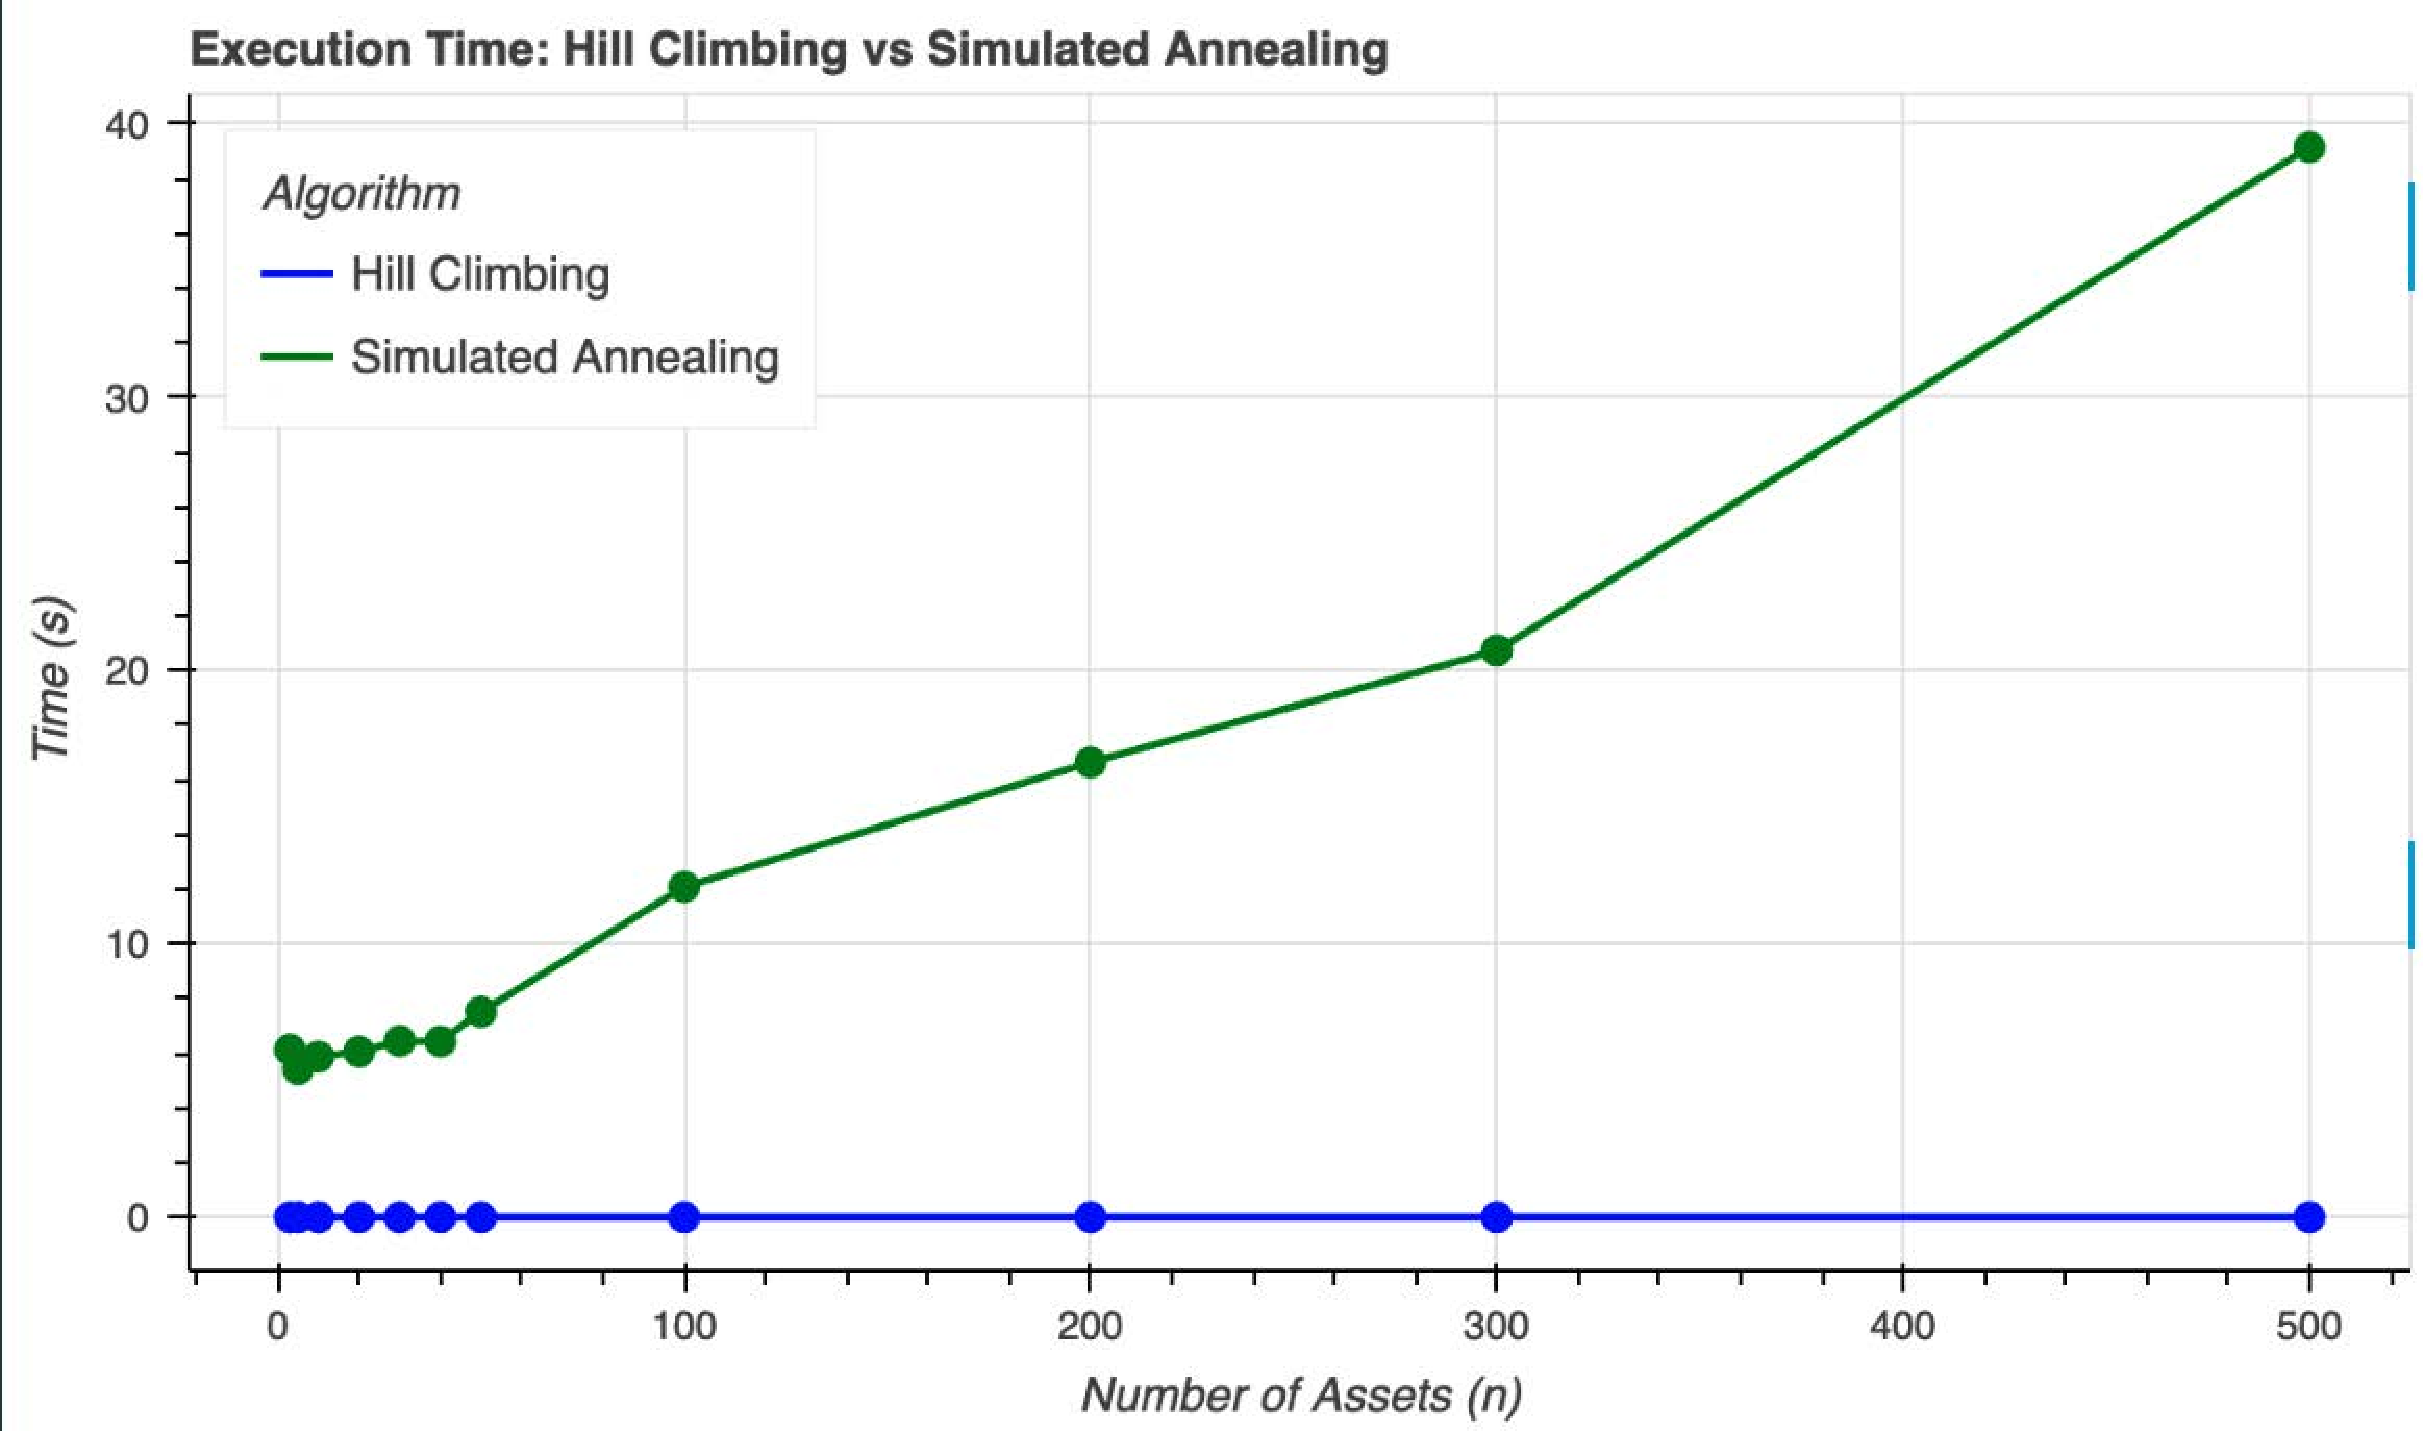
\includegraphics[width=\linewidth]{figures/exe_time.pdf}
            \caption{Grafica de comparación de tiempo de ejecuacion de Hill Climbing y Simulated Annealing}
            \label{fig:sample_figure}
        \end{figure}
        
        En la gráfica presentada se muestra la comparación del tiempo de ejecución entre dos algoritmos de optimización, Hill Climbing y Simulated Annealing, aplicados al problema de optimización de portafolios financieros. El eje horizontal representa el número de activos en el portafolio, mientras que el eje vertical indica el tiempo de ejecución en segundos, del resultado obtenido se puede deducir que Hill Climbing es constante y rápido en comparación con Simulated Annealing, porque este algoritmo no evalúa soluciones alternativas, en términos de tiempo de ejecución es más eficiente. Por otro lado, Simulated Annealing tiende a incrementar a medida que tenga más portafolios por analizar y esto se debe a que la naturaleza del algoritmo toma soluciones alternativas permitiendo descubrir el óptimo local y llegar hasta el óptimo global.


        %\begin{figure}[h]
        %    \centering
        %    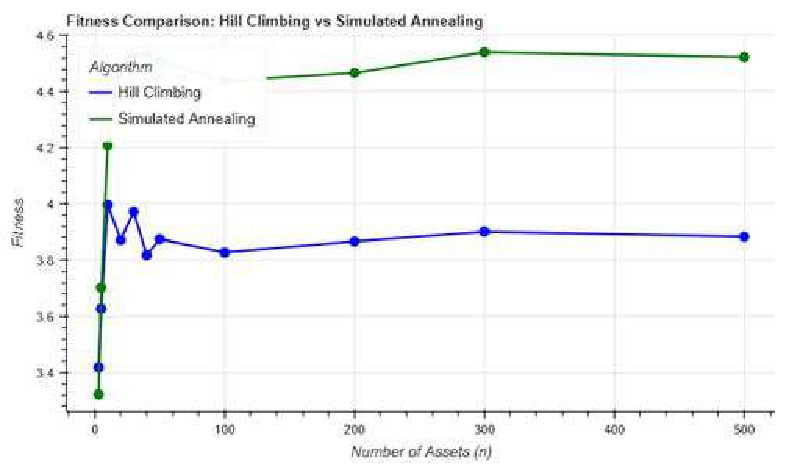
\includegraphics[width=\linewidth]{figures/exe_fitness.pdf}
        %    \caption{Grafica de comparación de resultados optimos Hill Climbing y Simulated Annealing para distintos tamaños de portafolio}
        %    \label{fig:sample_figure}
        %\end{figure}

        \begin{figure}[h]
            \centering
            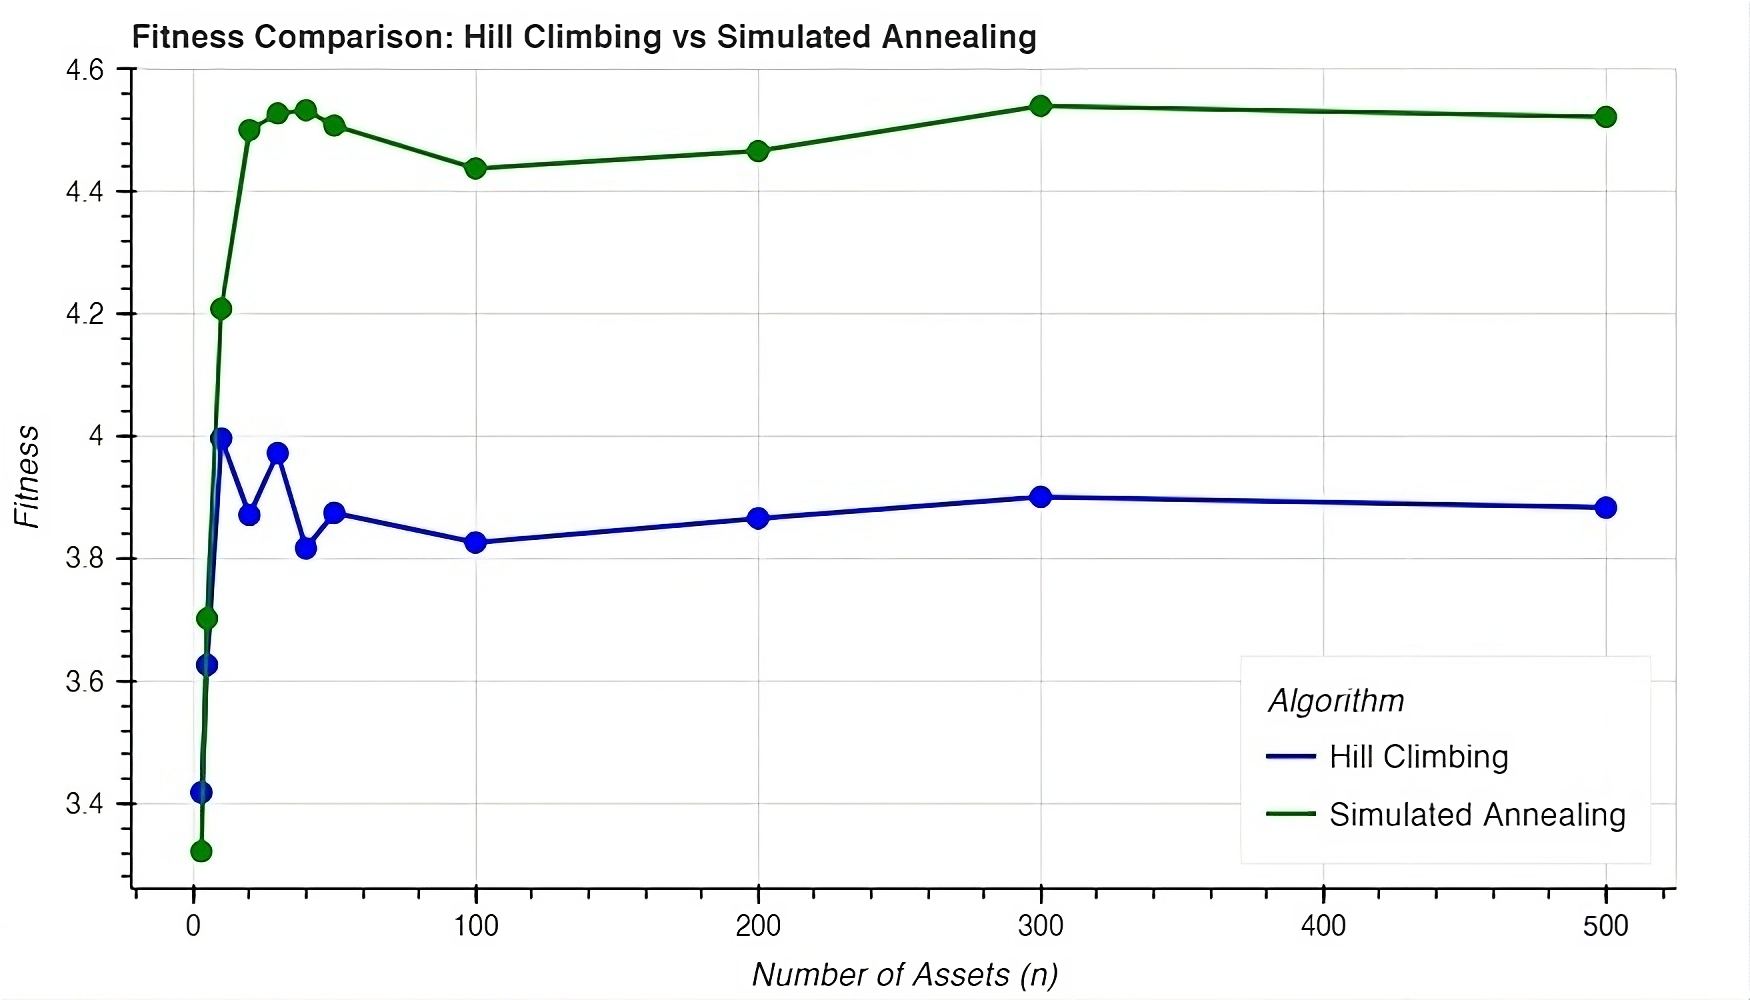
\includegraphics[width=\linewidth]{figures/Fitness_Comparisson-9x.png}
            \caption{Grafica de comparación de resultados optimos Hill Climbing y Simulated Annealing para distintos tamaños de portafolio}
            \label{fig:sample_figure2}
        \end{figure}

        La gráfica presentada muestra la comparación del fitness obtenido para el problema de optimización de portafolios utilizando dos algoritmos: Hill Climbing y Simulated Annealing. El eje horizontal representa el número de activos en el portafolio, y el eje vertical muestra el valor de fitness, medido como el ratio de Sharpe, que indica la relación entre el retorno esperado y el riesgo del portafolio. Del resultado obtenido se puede deducir que los valores fitness de Hill Climbing comparado con Simulated Annealing son bajos, debido a que es más probable que se quede atrapado en óptimos locales y no pueda explorar soluciones alternativas.
        



%----------------------------------------------------------
%----------------------------------------------------------
% CONCLUTIONS
%----------------------------------------------------------        
    \section{Conclusiones}
        \begin{itemize}
            \item \textbf{Impacto de los Parámetros en Simulated Annealing:} El rendimiento de \textbf{Simulated Annealing} depende de la configuración de la \textbf{temperatura inicial}, \textbf{temperatura mínima} y \textbf{tasa de enfriamiento}. Evaluar diferentes combinaciones de estos parámetros permite equilibrar la \textbf{exploración} y \textbf{explotación} del espacio de soluciones.

            \item \textbf{Evaluación de Robustez y Consistencia:} Evaluar la robustez de cada método ejecutándolos múltiples veces con distintas condiciones iniciales permite medir la variabilidad en los resultados. \textbf{Simulated Annealing} suele ser más consistente que \textbf{Hill Climbing} debido a su capacidad para escapar de óptimos locales.
            
            \item \textbf{Aplicabilidad para Portafolios Diversificados:} \textbf{Hill Climbing} es adecuado para soluciones rápidas y sencillas, mientras que \textbf{Simulated Annealing} es ideal para portafolios más diversificados donde se busca maximizar el rendimiento con una mayor diversidad de activos.
            
            \item \textbf{Adaptabilidad a Cambios del Mercado:} \textbf{Simulated Annealing} es más adaptable a las condiciones cambiantes del mercado debido a su enfoque estocástico, lo cual lo hace ideal para contextos con alta incertidumbre.
            
            \item \textbf{Aplicación Práctica y Escalabilidad:} \textbf{Hill Climbing} es adecuado para portafolios pequeños a medianos debido a su simplicidad. Para portafolios más grandes, \textbf{Simulated Annealing} ofrece mejores soluciones a pesar de requerir más tiempo de cálculo.
            
        \end{itemize}
%----------------------------------------------------------
% CONTENTS
%----------------------------------------------------------
    \renewcommand{\contentsname}{Tabla de Contenidos}
    \tableofcontents
    \linenumbers
%----------------------------------------------------------

\printbibliography

%----------------------------------------------------------    

\end{document}